\documentclass{article}
\usepackage[utf8]{inputenc}
\usepackage{geometry}
\usepackage{csquotes}
\usepackage[portuguese]{babel}
\usepackage[pdftex]{hyperref}
\usepackage{indentfirst}
\usepackage{tcolorbox}
\usepackage{amsmath}
\usepackage{tikz}

\tikzstyle{node} = [circle, draw = blue!50, fill = blue!20, thick, inner sep = 0pt, minimum size = 6mm]

\newtcolorbox{mybox}[3][]
{
  colframe = #2!25,
  colback  = #2!10,
  coltitle = #2!20!black,  
  title    = {#3},
  #1,
}

\geometry{top = 3cm, bottom = 2cm, right = 2cm, left = 3cm}
\title{PageRank e Cadeias de Markov}
\author{Cristhian Grundmann \\
Hanna Rodrigues Ferreira \\
Igor Cortes Junqueira \\
Igor Patrício Michels}

\date{Dezembro de 2021}

\begin{document}

\maketitle

\section*{Introdução}

Imagine que você esteja curioso acerca de um determinado tema, o que você faz? Se a resposta é ``dou um Google'', parabéns, você acaba de utilizar o algoritmo PageRank! Criado oficialmente em agosto de 1998, a Google surgiu com uma ideia de Larry Page e Sergey Brin. A história se inicia em 1995, quando Page foi conhecer a universidade de Stanford e Brin recebeu a tarefa de mostrar a universidade para ele. No início os dois discordavam sobre muita coisa mas, no ano seguinte, fecharam uma parceria visando criar um mecanismo de busca que pudesse ``organizar as informações do mundo e torná-las universalmente acessíveis e úteis''. Para isso, desenvolveram um algoritmo que usava os links para determinar a importância de cada página da internet \cite{google}.

Rapidamente o mecanismo ganhou força, virando o principal mecanismo de buscas. Esse fato se dá por que as estratégias de calcular a relevância, até o momento, eram calculadas usando apenas os dados da própria página, algo que poderia ser facilmente burlado e, com isso, poderia deixar resultados pouco relevantes nas primeiras posições, principalmente com o grande crescimento da internet na época.

\section*{Cadeias de Markov}

escrever uma historinha aqui
% falar que existe um estado estacionário se, e somente se, é aperiódica

\section*{PageRank}

Indo um pouco na contramão de algumas outras estratégias, o PageRank visa calcular a relevância de uma página por meio de fatores externos. De maneira simples, podemos usar um grafo para ilustrar uma pequena rede, onde os nós são os sites e as arestas, direcionadas, representam que o site de origem tem um link para o site de destino. É esperado que o site que receba a maior quantidade de links (maior grau de entrada) deve ser o mais relevante, mas e em caso de empate? A ideia de Page e Brin foi ponderar os votos de acordo com a relevância, isso é, se um site tem uma alta relevância, seu voto deve ter um peso maior que o voto de um site que não recebe link algum.
\begin{mybox}{green}{Exemplo}
    Um site que recebe apenas um link, mas do G1, deve ser mais relevante que um site que recebe apenas um link de um site pessoal.
\end{mybox}

\begin{figure}
    \centering
    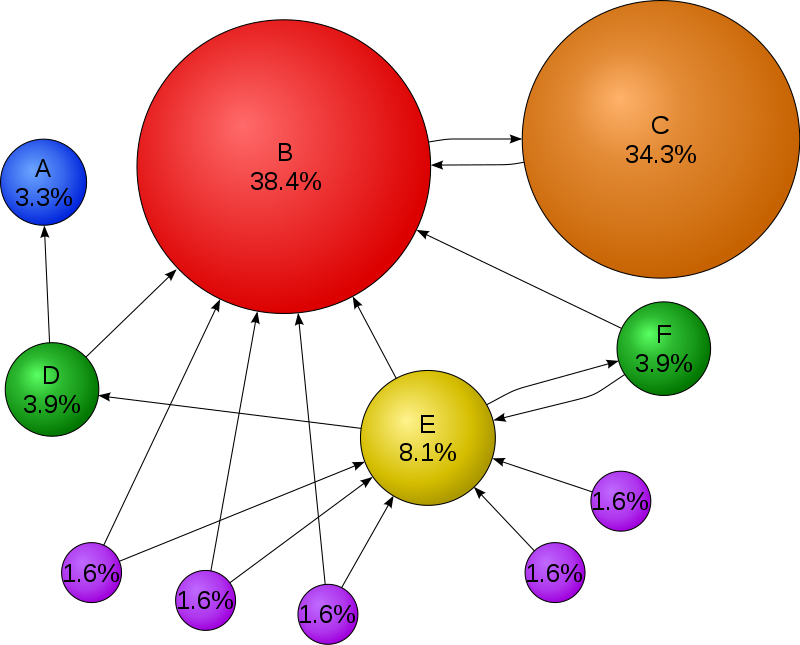
\includegraphics[scale = 0.5]{PageRanks-Example.png}
    \caption{Páginas e suas relevâncias. Note que, mesmo com apenas um ``voto'', a página C tem uma alta relevância. Exemplo de \cite{wiki}.}
    \label{wiki_example}
\end{figure}

\subsection*{Conexão com as Cadeias de Markov}

Intuitivamente, podemos pensar no processo de um internauta ficar navegando na internet e trocar de sites por meio de links presentes no próprio site, com mesma probabilidade para cada link. Dessa forma, se um site $S$ tem link para $n$ diferentes sites ($T_1$, $T_2$, $\dots$ e $T_n$), a probabilidade do internauta sair do site $S$ para os sites $T_i, i \in \{1, 2, \dots, n\}$ é igual a $\frac{1}{n}$ e é nula para qualquer outro site.

Note que temos uma modelagem concisa que representa a rede de modo simples resta, então, definir uma métrica para representar a relevância de um site. Pensando em Cadeias de Markov, com sua evolução temporal, podemos pensar que uma boa métrica seja dada pela proporção do tempo que o internauta aleatório passa em cada site, ou seja, é maior para sites mais recorrentes e menor para sites menos visitados. Note que essa definição é coerente com a ideia de que sites mais relevantes tenham votos mais significativos.

\subsection*{Tratando as entradas nulas e implementando}

\begin{tikzpicture}
    \node (A) at (0, 1.7) [node] {};
    \node (B) at (-1, 0) [node] {};
    \node (C) at (1, 0) [node] {};
    \draw [->] (A) -- (B);
    \draw [->] (B) -- (C);
    \draw [->] (C) -- (A);
    
    \node (D) at (5, 1.7) [node] {};
    \node (E) at (5, 0.85) [node] {};
    \node (F) at (5, 0) [node] {};
    \node (G) at (7, 0.85) [node] {};
    \draw [->] (D) -- (G);
    \draw [->] (E) -- (G);
    \draw [->] (F) -- (G);
\end{tikzpicture}

Como vimos anteriormente, podemos modelar as transições entre dois sites por meio de uma Cadeia de Markov. Porém, como sabemos, nem todos os sites recebem links de todos os outros sites (na verdade, a grande maioria nem se conecta), ou seja, nossa matriz de transição da cadeia é esparsa e pode não existir distribuição estacionária para essa cadeia. Uma forma de resolver esse problema é adicionar links fictícios entre todos os sites, mas de modo que esses links somem uma probabilidade baixa. Dessa forma, temos a seguinte matriz da cadeia
\[M = (1 - p)\cdot A + p\cdot \dfrac{I}{n},\]

\noindent onde temos
\begin{itemize}
    \item
        $M$: a matriz de transição da cadeia;
        
    \item
        $p$: a probabilidade de entrar em um site aleatório;
        
    \item
        $A$: a matriz de adjacências da rede;
        
    \item
        $I$: a matriz de uns de tamanho $n\times n$ e;
        
    \item
        $n$: o número de nós da rede.
\end{itemize}

\newpage
\begin{thebibliography}{9}

\bibitem{google} Como nós começamos e onde estamos hoje. \textit{Google}. \url{https://about.google/our-story/}.

\bibitem{usp} O algoritmo PageRank do Google. \textit{Miguel Frasson - ICMC/USP}. \url{https://edisciplinas.usp.br/pluginfile.php/5790758/mod_resource/content/1/pagerank-estat.pdf}.

\bibitem{wiki} ``PageRank''. \textit{Wikipedia}. \url{https://en.wikipedia.org/wiki/PageRank}.

\end{thebibliography}

\end{document}

